\documentclass[12pt]{article}
\usepackage[utf8]{inputenc}
\usepackage{amsmath}
\usepackage{amsfonts}
\usepackage{amssymb}
\usepackage{graphicx}
\usepackage{hyperref}
\usepackage{subcaption}
\usepackage{tocloft}

\renewcommand{\cftsecleader}{\cftdotfill{\cftdotsep}} % for sections
\newcommand*{\Nvidia}{\textsc{NVIDIA}}
\newcommand*{\GeForce}{\textsc{GeForce}}
\newcommand*{\Cuda}{\textsc{CUDA}}
\newcommand*{\OpenCV}{\textsc{OpenCV}}
\newcommand*{\OpenGL}{\textsc{OpenGL}}

\usepackage[dvipsnames]{xcolor}
\colorlet{mygray}{black!30}
\colorlet{mygreen}{green!60!blue}
\colorlet{mymauve}{red!60!blue}
\usepackage{listings}
\lstset{
	escapeinside={<@}{@>},
	backgroundcolor=\color{gray!5},
	basicstyle=\ttfamily\footnotesize,
	columns=fullflexible,
	breakatwhitespace=false,
	breaklines=true,
	captionpos=b,
	aboveskip=1em,belowskip=-1em,
	commentstyle=\color{mygreen},
	extendedchars=true,
	frame=single,
	keepspaces=true,
	keywordstyle=\color{blue},
	language=[ANSI]C++,
	numbers=left,
	numbersep=5pt,
	numberstyle=\tiny\color{blue},
	rulecolor=\color{mygray},
	showspaces=false,
	showtabs=false,
	showstringspaces=false
	stepnumber=1,
	stringstyle=\color{mymauve},
	tabsize=3,
	title=\lstname
}
\lstdefinestyle{DOS}
{
	backgroundcolor=\color{gray!5},
	numbers=none,
	stringstyle=\color{black},
}
\usepackage[margin=2cm]{geometry}
\author{Davide Stocco}
\title{
  \textbf{Radial Undistortion of Images}\\
	\Nvidia{} \Cuda{} Parallel Processing\\
	\vspace{0.2in}
	\large{\Cuda{} Toolkit 9.1 - December 2017 Release\\
	\vspace{0.02in}
	\Nvidia{} \GeForce{} 840M (Performance Score 5.0x)}
}
%
\begin{document}
\maketitle
\vfill
\tableofcontents
\pagebreak
%
\section{Introduction}

This project is focused on speeding up a radial distortion correction of a camera capture. The reason behind this is to reach a high computational speed so that further operations can also be performed in real-time while video capturing. To reach such a target we will parallelize undistortion operations by means of an \Nvidia{} GPU (\emph{Graphics Processing Unit}). This GPU is provided with a \Cuda{} (\emph{Compute Unified Device Architecture}) accelerator that consists of a high number of threads in which to split and complete the task in less time. In other words, starting from an image frame, \OpenCV{} will convert it into a $M \times N$ \texttt{Mat} class dense array. Then the \texttt{Mat.data} substructure will be allocated in the \Cuda{} device memory as a $1 \times (M \times N)$ array and undistorted by the \Cuda{} kernel. When the undistortion process is done the data will be sent back to the host device memory (RAM) and converted again on an \OpenCV{} $M \times N$ \texttt{Mat} class dense array.

\section{Radial Distortion}

Radial distortion is a phenomenon that deforms an image. This unwanted but unavoidable phenomenon is due to a deviation from the rectilinear projection of light and it is a form of optical aberration. Radial distortion is a big set of different kinds of distortions and it can be furtherly classified as:
%
\begin{itemize}
	\setlength\itemsep{0em}
	\item \textit{barrel} distortion;
	\item \textit{pincushion} distortion;
	\item \textit{mustache} distortion.
\end{itemize}
%
\begin{figure}[h!]
	\centering
	\begin{subfigure}{0.30\linewidth}
		\centering
		\frame{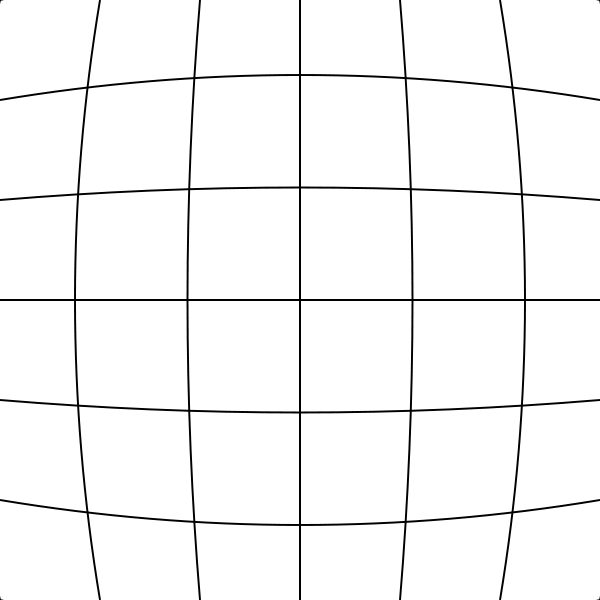
\includegraphics[width=\linewidth]{./figures/barrel.png}}
		\caption{Barrel distortion}
		\label{barrel}
	\end{subfigure}\hfill
	\begin{subfigure}{0.30\linewidth}
		\centering
		\frame{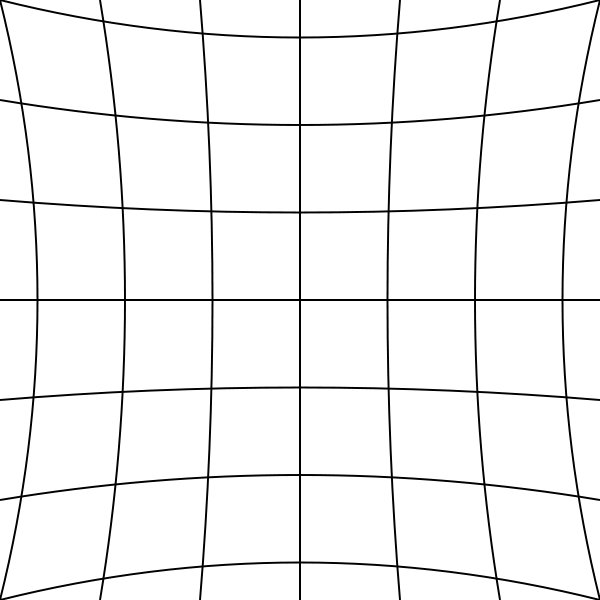
\includegraphics[width=\linewidth]{./figures/pincushion.png}}
		\caption{Pincushion distortion}
		\label{pincushion}
	\end{subfigure}\hfill
	\begin{subfigure}{0.30\linewidth}
		\centering
		\frame{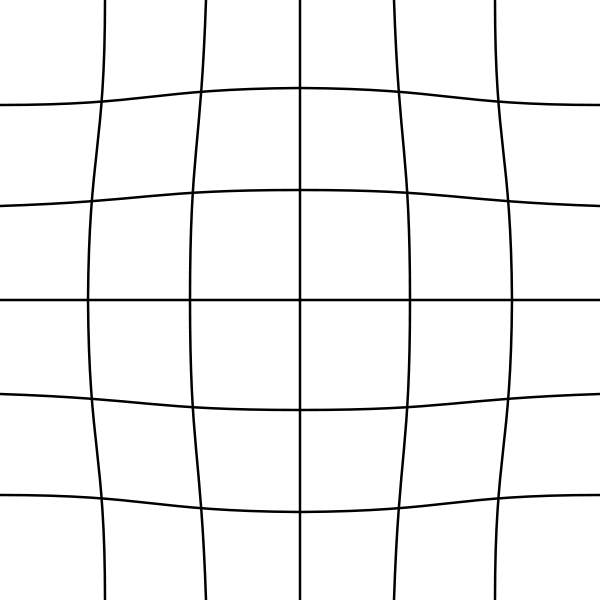
\includegraphics[width=\linewidth]{./figures/mustache.png}}
		\caption{Mustache distortion}
		\label{mustache}
	\end{subfigure}
	\caption{Different types of radial distortion.}
	\label{types}
\end{figure}
%
Mathematically, barrel and pincushion distortion are \textit{quadratic}, meaning they increase as the square of the distance from the centre. In moustache distortion the \textit{quartic} term is significant: in the centre, the degree two barrel distortion is dominant, while at the edge the degree four distortions in the pincushion direction dominate. In this discussion, we will only focus on barrel and pincushion distortion.

\subsection{Software Correction}

Radial distortion can be corrected by using the \textit{Brown-Conrady model}. This model corrects both radial and tangential distortions caused by misaligned elements in a lens. The most commonly used distortion correction model in software is known as \textit{decentering distortion model}, and it can be expressed in mathematical form as:
%
\begin{equation}
  \begin{split}
    x_u =\ & x_{d}+\dots \\
    &(x_d-x_c)(K_{1}r^{2}+K_{2}r^{4}+\dots )+\dots \\
    &(P_{1}(r^{2}+2(x_d-x_c)^{2})+2P_{2}(x_d-x_c)(y_d-y_c))(1+P_{3}r^{2}+P_{4}r^{4}\dots
  \end{split}
\end{equation}
%
\begin{equation}
  \begin{split}
    y_u =\ & y_d+\dots \\
    &(y_d-y_c)(K_{1}r^{2}+K_{2}r^{4}+\dots )+\dots \\
    &(2P_{1}(x_d-x_c)(y_d-y_c)P_{2}(r^{2}+2(y_d-y_c)^{2}))(1+P_{3}r^{2}+P_{4}r^{4}\dots
  \end{split}
\end{equation}
%
where:
%
\begin{itemize}
	\setlength\itemsep{0em}
	\item $(x_d, y_d)$ is the distorted image point;
	\item $(x_u, y_u)$ is the undistorted image point;
	\item $(x_c, y_c)$ is the distortion center;
	\item $K_n$ is the $n$-th \textit{radial distortion coefficient};
	\item $P_n$ is the $n$-th \textit{tangential distortion coefficient};
	\item $r = \sqrt{(x_d-x_c)^2+(y_d-y_c)^2}$.
\end{itemize}
%
Each kind of distortion has a typical sign and value of the $K_n$ and $P_n$ terms, hence they can be characterized accordingly.

\subsection{Inverse Model Approach for Radial Distortion Correction}

The Brown-Conrady model is non-linear, and thus also not invertible. To invert such a non-linear model we would need a numeric approach, which is quite precise but not as fast as we would it to be. Pierre Drap and Julien Lefèvre in \cite{model} proposed an \textit{original approach} which aims us to compute the inverse transformation of a pure radial distortion model\footnote{ Pure radial distortion model is characterized by $P_n = 0$ with $n = 1,\dots,n$.}.

Given a model of distortion or correction with parameters $(k_1,k_2,k_3,\dots)$, they expressed the inverse transformation on the same form of the direct transformation, i.e. with parameters $(k'_1,k'_2,k'_3,\dots)$. Therefore they expressed each $k'_i$ as a function of all the $k_j$. More practically, given the generic transformation $T$, they demonstrate that:
%
\begin{equation}
  T:
  \begin{pmatrix}
    x_u \\
    y_u
  \end{pmatrix}
  \rightarrow
  \begin{pmatrix}
    x_d \\
    y_d
  \end{pmatrix}
  = Q(r^\prime)
  \begin{pmatrix}
    x_u \\
    y_u
  \end{pmatrix}
\end{equation}
%
where $r^\prime = \sqrt{(x_u-x_c)^2+(y_u-y_c)^2}$ and $Q(r^\prime)$ can be expressed as a power series that authors have demonstrated to be:
%
\begin{equation}
  Q(r^\prime)=\sum_{n=0}^{+\infty}b_n (r^\prime)^{2n}
  \label{Q}.
\end{equation}
%
Drap and Lefèvre also found a recursive formula to compute $b_n$ terms as a function of distortion or correction parameters $(-k_1,-k_2,-k_3,\dots)$. For this application we will stop at the first four terms, which are:
%
\begin{equation}
  \begin{split}
    b_1 &= - k_1 \\
    b_2 &= 3 k_1^2 - k2 \\
    b_3 &= - 12 k_1^3 + 8 k_1 k_2 - k_3 \\
    b_4 &= 55 k_1^4 - 55 k_1^2 k_2+ 5 k_2^2 + 10 k_1 k_3 - k_4.
  \end{split}
\end{equation}

\subsection{Advantages of the Inverse Algorithm}

An example of the final result of the distortion or correction process using the Brown-Conrady model is shown in \figurename{ \ref{exlena}}. Notice that black lines appear on the most stretched sides of the image. This phenomenon occurs when the remapping operation shifts pixels by a distance which in modulus is bigger than a unit. Unluckily, this kind of visual artefact cannot be avoided and further software corrections are needed in order to interpolate pixel values in the surroundings of holes.
%
\begin{figure}
	\centering
	\begin{subfigure}{0.30\linewidth}
		\centering
		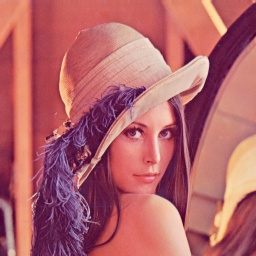
\includegraphics[width=\linewidth]{./figures/lena.jpg}
		\caption{Original image}
		\label{lena01}
	\end{subfigure}\hfill
	\begin{subfigure}{0.30\linewidth}
		\centering
		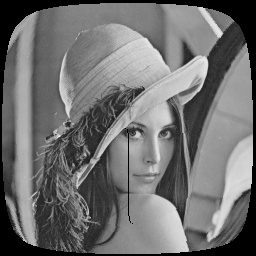
\includegraphics[width=\linewidth]{./figures/lena1.jpg}
		\caption{Barrel distortion}
		\label{lena11}
	\end{subfigure}\hfill
	\begin{subfigure}{0.30\linewidth}
		\centering
		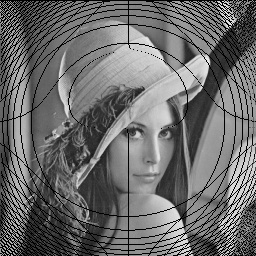
\includegraphics[width=\linewidth]{./figures/lena2.jpg}
		\caption{Pincushion distortion}
		\label{lena21}
	\end{subfigure}
	\caption{Distortion of a sample image using Brown-Conrady model. Notice the visual artefacts that occur not only when applying pincushion distortion (\figurename{ \ref{lena11}}) but also when applying barrel distortion with a light tangential distortion (\figurename{ \ref{lena21}}).}
	\label{exlena}
\end{figure}
%
The main advantage of the inverse approach is that starting from the destination or corrected image and by the inverse transformation, we can compute the a priori position of each pixel. With this method every pixel of the destination image is mapped to its original position in the source or distorted image, the result is that no empty spaces or visual artefacts are left in the corrected image.
%
\begin{figure}[h!]
	\centering
	\begin{subfigure}{0.30\linewidth}
		\centering
		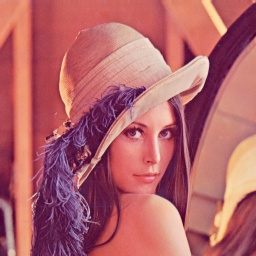
\includegraphics[width=\linewidth]{./figures/lena.jpg}
		\caption{Original image}
		\label{lena02}
	\end{subfigure}\hfill
	\begin{subfigure}{0.30\linewidth}
		\centering
		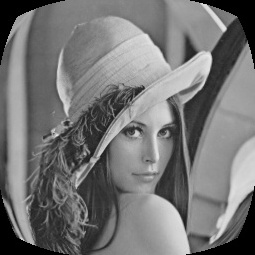
\includegraphics[width=\linewidth]{./figures/lena11.jpg}
		\caption{Barrel distortion}
		\label{lena12}
	\end{subfigure}\hfill
	\begin{subfigure}{0.30\linewidth}
		\centering
		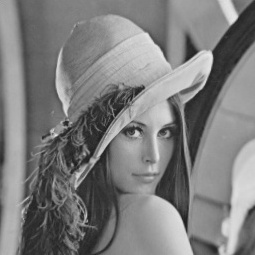
\includegraphics[width=\linewidth]{./figures/lena21.jpg}
		\caption{Pincushion distortion}
		\label{lena22}
	\end{subfigure}
	\caption{Distortion of a sample image using the inverse model proposed by Pierre Drap and Julien Lefèvre in \cite{model}. Notice that visual artefacts disappear.}
	\label{exlena_approx}
\end{figure}

\subsection{Bilinear Interpolation}

In computer vision and image processing, bilinear interpolation is one of the basic resampling techniques. When an image needs to be scaled up, each pixel of the original image needs to be moved in a certain direction based on the scale constant. However, when scaling up an image by a non-integer scale factor, some pixels are not assigned appropriate pixel values. In this case, those holes should be assigned appropriate RGB or grayscale values so that the output image does not have non-valued pixels.

Bilinear interpolation can be used where perfect image transformation with pixel matching is impossible so that one can calculate and assign appropriate intensity values to pixels. Unlike other interpolation techniques such as nearest-neighbour interpolation and bi-cubic interpolation, bilinear interpolation uses values of only the four nearest pixels, located in diagonal directions from a given pixel, in order to find the appropriate colour intensity values of that pixel.

Bilinear interpolation considers the closest $2 \times 2$ neighbourhood of known pixel intensity values surrounding the unknown pixel's computed location as:
%
\begin{equation}
  \begin{aligned}
  I(x,y_{1})\approx {\frac {x_{2}-x}{x_{2}-x_{1}}}I_{11}+{\frac {x-x_{1}}{x_{2}-x_{1}}}I_{21} \\
  I(x,y_{2})\approx {\frac {x_{2}-x}{x_{2}-x_{1}}}I_{12}+{\frac {x-x_{1}}{x_{2}-x_{1}}}I_{22}.
  \end{aligned}
\end{equation}
%
It then takes a weighted average of these four pixels to arrive at its final, interpolated value:
\begin{equation}
  I(x,y)\approx {\frac {y_{2}-y}{y_{2}-y_{1}}}I(x,y_{1})+{\frac {y-y_{1}}{y_{2}-y_{1}}}I(x,y_{2}).
\end{equation}
%
\begin{figure}[h!]
	\centering
	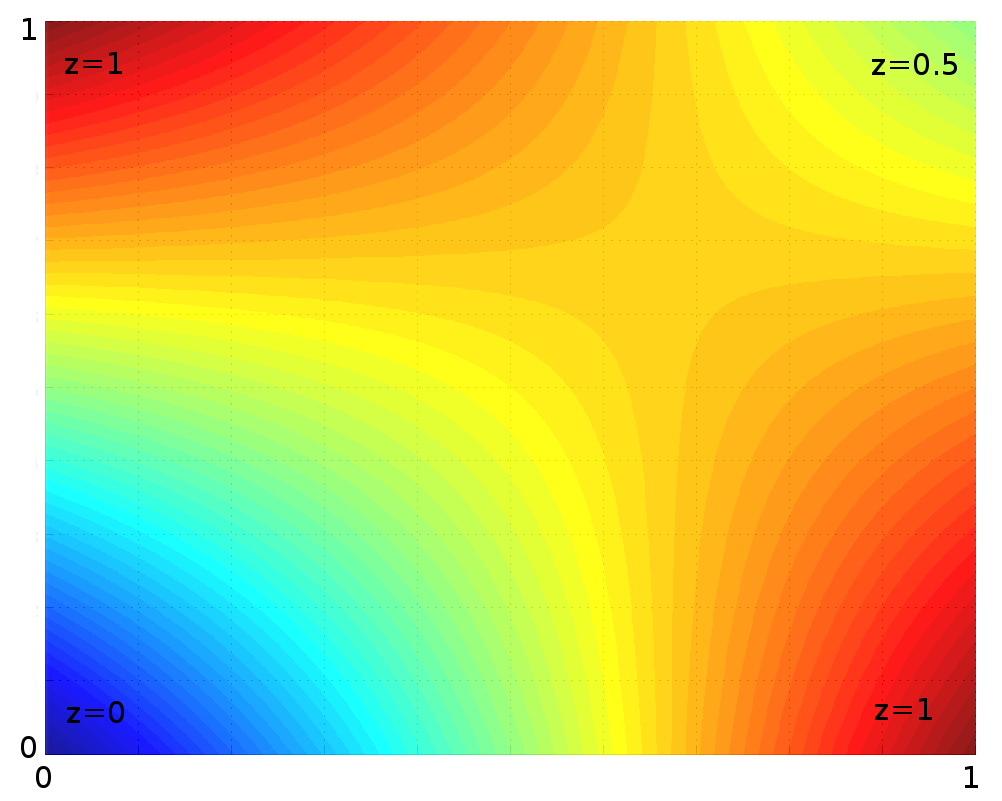
\includegraphics[width=0.4\linewidth]{figures/bilininterp}
	\caption{Example of bilinear interpolation on the unit square with $z$ values equal to $0$, $1$, $1$ and $0.5$. Interpolated values in between are represented by colour shades.}
	\label{fig:bilininterp}
\end{figure}
%
\section{\Cuda{} Background}
%
\subsection{History of \Cuda{}}
Driven by the market demand for real-time and high-definition graphics, the programmable GPU has evolved into a highly parallel, multi-threaded and multi-core processor with high computational power and large memory bandwidth. More specifically, the GPU is especially well suited to address problems that can be expressed as \textit{data-parallel computations}\footnote{ The same program is executed on many data elements in parallel.} with \textit{high arithmetic intensity}\footnote{ The ratio of arithmetic operations to memory operations.}. Because the same program is executed for each data element, there is a lower requirement for sophisticated flow control, and because it is executed on many data elements and has high arithmetic intensity, the memory access latency can be hidden with calculations instead of big data caches. Data-parallel processing maps data elements to parallel processing threads. Many applications that process large data sets can use a data-parallel programming model to speed up the computations.

\Cuda{} was introduced by \Nvidia{} in 2006 as a general-purpose parallel computing platform and programming model. It uses the parallel computing engine in \Nvidia{} GPUs to solve many complex computational problems in a more efficient way than on a CPU.

\subsection{\Cuda{} GPUs}

The advent of multi-core CPUs and many-core GPUs means that mainstream processor chips are now parallel systems. The challenge is to develop application software that scales its parallelism to exploit the increasing number of processor cores. The \Cuda{} parallel programming model is designed to overcome this challenge while maintaining a low learning curve for programmers familiar with standard programming languages such as C. At its core, there are three key abstractions\footnote{ A hierarchy of thread groups, shared memories, and barrier synchronization.} that are simply exposed to the programmer as a minimal set of language extensions. These abstractions provide fine-grained \textit{data parallelism} and \textit{thread parallelism}, nested within coarse-grained \textit{data parallelism} and \textit{task parallelism}. They guide the programmer to partition the problem into coarse sub-problems that can be solved independently in parallel by blocks of threads, and each sub-problem into finer pieces that can be solved cooperatively in parallel by all threads within the block.

This decomposition preserves language expressivity by allowing threads to cooperate when solving each sub-problem, and at the same time enables automatic scalability. Indeed, each block of threads can be scheduled on any of the available multiprocessors within a GPU, in any order, \textit{concurrently} or \textit{sequentially}, so that a compiled \Cuda{} program can execute on any number of multiprocessors, and only the runtime system needs to know the physical multiprocessor count.
%
\subsection{Advantages and Limitations}
\Cuda{} has advantages over traditional General-Purpose computation on GPUs (GPGPU) using graphics APIs:
\begin{itemize}
	\setlength\itemsep{0em}
	\item scattered reads\footnote{ Code can read from arbitrary addresses in memory.};
	\item unified virtual memory;
	\item unified memory;
	\item fast shared memory among threads;
	\item faster downloads and read-backs to and from the GPU;
	\item full support for integer and bitwise operations, including integer texture lookups.
\end{itemize}
But it has some disadvantages too:
\begin{itemize}
	\setlength\itemsep{0em}
	\item limited interoperability \footnote{ Interoperability with other languages such as \OpenGL{} is one-way, with \OpenGL{} having access to registered \Cuda{} memory but \Cuda{} not having access to \OpenGL{} memory.}
	\item copying between host and device memory may incur a performance hit due to system bus bandwidth and latency\footnote{ This can be partly alleviated with asynchronous memory transfers.};
	\item threads should be running in groups of at least 32 for best performance.
\end{itemize}

\section{\Cuda{} Coding}

In this section, the \Cuda{} kernel code and related parts to undistort or correct images will be described.

\subsection{\Cuda{} Error Checking}

Checking the results returned by \Cuda{} API functions is important to ensure getting \texttt{cudaSuccess}, which means that the API call is returned with no errors.

\begin{lstlisting}
// \Cuda{} error check
inline
void
GPU_Assert(
  cudaError_t code,         // Error code
  const char *file,         // File name
  int         line,         // Line number
  bool        abort = false // Abort program flag
)
{
  if (code != cudaSuccess)
  {
    fprintf(stderr, "GPUassert: \%s \%s \%d\n", cudaGetErrorString(code), file, line);
    if (abort == true)
      exit(code);
  }
}
\end{lstlisting}

As it can be seen, the error checking function \texttt{GPU\_Assert} only needs the \Cuda{} command as input and it will print a string of the form ``\texttt{GPUassert: \#Type\_of\_error \#File \#Line\_number}''. It also can be chosen whether to abort or continue the execution of the program if an error occurs.

\subsection{\Cuda{} Kernel}

The \Cuda{} kernel is the core of the program, it defines the GPU tasks and how to perform these tasks. \Cuda{} kernels must be declared before any host function.
%
\begin{lstlisting}
// \Cuda{} kernel for undistortion
<@\textcolor{mymauve}{\_\_global\_\_}@>
void
undistort(
  uchar *image_in,     // Input image
  uchar *image_out_CUDA, // Output image
  double k1,        // Radial distortion coefficient k1
  double k2,        // Radial distortion coefficient k2
  double k3,        // Radial distortion coefficient k3
  double k4,        // Radial distortion coefficient k4
  int    width,     // Image width
  int    height     // Image height
)
{
  // Setting texture memory
  uint i = blockIdx.x * blockDim.x + threadIdx.x ;
  uint j = blockIdx.y * blockDim.y + threadIdx.y;

  // Define distortion center and polar coordinates
  double xc = width / 2.0;
  double yc = height / 2.0;
  double r  = std::sqrt((i-xc)*(i-xc) + (j-yc)*(j-yc));

  double k1_2 = k1*k1;
  double r_2  = r*r;
  double r_4  = r_2*r_2;

  // Calculate bn coefficents and Inverse transformation Q
  // Notice that b0 = 1
  double b1 = -k1;
  double b2 = 3.0*k1_2 - k2;
  double b3 = 8.0*k1*k2 - 12.0*k1_2*k1 - k3;
  double b4 = 55.0*k1_2*k1_2 + 10.0*k1*k3 - 55.0*k1_2*k2 + 5*k2*k2 - k4;
  double Q  = 1.0 + b1*r_2 + b2*r_4 + b3*r_2*r_4 + b4*r_4*r_4;

  // Final (x,y) coordinates
  double x = (i-xc) * Q;
  double y = (j-yc) * Q;
  int    o = xc + yc * width;

  // Bilinear Interpolation Algorithm
  // Ensure that the undistorted point sits in the image
  if (i <= width && j <= height)
  {
    // Define intermediate points
    int x1 = std::floor(x);
    int y1 = std::floor(y);
    int x2 = x1 + 1;
    int y2 = y1 + 1;

    // Ensure that the mean color value is computable
    if(x1 >= -xc && y1 >= -yc && x2 < (width/2.0) && y2 < (height/2.0))
    {
      double val1 = image_in[x1 + y1 * width + o];
      double val2 = image_in[x2 + y1 * width + o];
      double val3 = image_in[x1 + y2 * width + o];
      double val4 = image_in[x2 + y2 * width + o];

      double color1 = (x2 - x) * val1 + (x - x1) * val2;
      double color2 = (x2 - x) * val3 + (x - x1) * val4;

      image_out_CUDA[i + j * width] = (y2 - y) * color1 + (y - y1) * color2;
    }
  }
}
\end{lstlisting}
%
In the first part the \texttt{undistort} function is introduced as a \texttt{\_\_global\_\_} kernel\footnote{ In \Cuda{} there are two types of functions, \texttt{\_\_global\_\_} functions (or kernels), which can be called from host code by the call semantics (\texttt{<<<\dots>>>}), and \texttt{\_\_device\_\_} functions, which cannot be called from host code.}. The inputs are the two \texttt{Mat.data} substructure arrays, the first contains the source image while the second is a zero-valued array (black image) which will be overwritten in the remapping process. Both \texttt{Mat.data} are automatically given in a $1 \times (M \times N)$ layout. Other inputs are the distortion values and the two dimensions of the image.

\textit{Texture memory} defines the indexing order, or in other words in which order to perform the remapping process. In this case, the kernel will subdivide the image in a 2D texture of $\texttt{blockDim.x}\times\texttt{blockDim.y}$ windows dimensions and will address each pixel to a specific thread.

Final coordinates are defined as integer numbers because they will correspond to a specific pixel position in the final image. Distortion centre is initialized as a float for straightforwardness\footnote{ It would be anyway converted to a float number within \texttt{powf} and \texttt{sqrtf} functions.}. Then the \textit{inverse remapping process} starts with the calculation of the \texttt{r} coefficient. By using the formula given in \eqref{Q} and $b_n$ coefficients, the original position of each pixel in the undistorted or corrected image is computed. Of course, the position will not be an integer and the colour intensity value is computed through the previously presented bilinear interpolation algorithm.
%
\subsection{Main Function}
%
The \texttt{main} function consists of a \texttt{while} loop that will ask for distortion parameters modifications and will return the output image until the exit key is given on the command window. More specifically, a \texttt{switch} function will do the job. In this section of the code distortion parameters \texttt{k1}, \texttt{k2}, \texttt{k3} and \texttt{k4} can be increased, decreased, reset to zero and shown in the command window.
%
\subsubsection{System Variables Allocation}
%
\begin{lstlisting}
// Read input image
Mat image_in = imread("path-to-image-file", 0);
uchar *img_in;

// Allocate output image
Mat image_out_CUDA = Mat(image_in.rows, image_in.cols, CV_8UC1, double(0.0));
uchar *img_out;

// Get image size
int N = image_in.rows * image_in.cols;

// Initialize \Cuda{} stream and error
cudaStream_t CUDA_stream;
cudaError_t  CUDA_error;
CUDA_error = cudaStreamCreate(&CUDA_stream);

// To GPU memory
GPU_ERROR(cudaFree(0));
GPU_ERROR(cudaMalloc(&img_in, N*sizeof(uchar)));
GPU_ERROR(cudaMemcpyAsync(img_in, image_in.data, N*sizeof(uchar), cudaMemcpyHostToDevice, CUDA_stream));
GPU_ERROR(cudaMalloc(&img_out, N*sizeof(uchar)));
GPU_ERROR(cudaMemcpyAsync(img_out, image_out_CUDA.data, N*sizeof(uchar), cudaMemcpyHostToDevice, CUDA_stream));
\end{lstlisting}
%
The source image is transformed into one channel \texttt{CV\_8UC1} \texttt{Mat} dense class array and an \texttt{img} pointer are initialized. The same is done also for the zero-valued \texttt{Mat}. A \Cuda{} stream is launched and the allocation of data in the GPU starts by means of \texttt{cudaMalloc} function. Then the data is copied from the RAM to the GPU memory through \texttt{cudaMemcpyAsync} function which specifies the source data, the destination pointer, the direction of data flow (in this case \texttt{cudaMemcpyHostToDevice}) and in which stream it operates.
%
\subsubsection{Kernel Settings, Launch and Output Error Checking}
%
\begin{lstlisting}
// Kernel settings
dim3 dimBlock(256, 540);
dim3 numBlocks(image_in.cols/dimBlock.x, image_in.rows/dimBlock.y);

// Apply kernel on input image
clock_t CUDA_start_clock = clock();
undistort<<<dimBlock, numBlocks, 0, CUDA_stream>>>(
  img_in, img_out, k1, k2, k3, k4, image_in.cols, image_in.rows
  );
cudaDeviceSynchronize();
GPU_ERROR(cudaPeekAtLastError());
clock_t CUDA_stop_clock = clock();
double CUDA_elapsed_time =
  (CUDA_stop_clock - CUDA_start_clock) * 1000.0 / (double)CLOCKS_PER_SEC;

std::cout
  << "Custom \Cuda{} kernel - Elapsed time:"
  << CUDA_elapsed_time << " (ms)" << std::endl;
GPU_ERROR(cudaPeekAtLastError());

// Check for \Cuda{} errors
cudaError_t CUDA_past_error = cudaGetLastError();
if (CUDA_past_error != cudaSuccess)
{
  fprintf(stderr, "\Cuda{} ERROR: \%s \n", cudaGetErrorString(CUDA_past_error));
}
\end{lstlisting}
%
Dimensions of block texture in which to subdivide the capture are arbitrarily decided through \texttt{dimBlock} function\footnote{ Actually, the function \texttt{dimBlock} specifies the number of threads per block. In this application, thread IDs correspond with pixels, so the numbers given in \texttt{dimBlock} function correspond to the pixel dimensions of the window in which to subdivide the source frame.}, while the calculation of blocks number is automatized. After setting these parameters, the \texttt{undistort} is called and inputs are given accordingly.

Further \Cuda{} error checking is performed and \texttt{cudaPeekAtLastError} returns the last error that has been produced by any of the runtime calls in the same host thread. Possible errors on the stream are also checked.

The execution time of the kernel is a key factor for evaluating performance. Thus, it is measured from kernel invoking to the end of \texttt{cudaDeviceSynchronize()}, which waits for every thread and block to finish before stopping the timer.

\subsubsection{Copy Data from GPU Memory to RAM}

\begin{lstlisting}
// To CPU
uchar * out = (uchar*)malloc(N * sizeof(uchar));
GPU_ERROR(cudaMemcpyAsync(out, img_out, N * sizeof(uchar), cudaMemcpyDeviceToHost, CUDA_stream));
Mat out_Mat = Mat(image_in.rows, image_in.cols, CV_8UC1, out);
\end{lstlisting}
%
In the final part of the code the $1 \times (M\times N)$ output array is copied from GPU memory to RAM through \texttt{cudaMemcpyAsync} function and now the data flow is defined as \texttt{cudaMemcpyDevice}-\texttt{ToHost}. Finally, the data is converted again in one channel $M\times N$ \texttt{Mat} array.
%
\section{Code Execution and Results}
%
Code execution is performed through a properly integrated development environment (Microsoft Visual Studio). Here is an example of what appears in the command window during execution.
%
\begin{lstlisting}[style=DOS]
\Cuda{} KERNEL FOR RADIAL UNDISTORTION
Press key:
'a'=+k1 'z'=-k1 's'=+k2 'x'=+k2
'd'=+k3 'c'=-k3 'f'=+k4 'v'=+k4
'w' = See current distortion values
'r' = Reset distortion values
'q' = Quit program

Key:    a
Custom \Cuda{} kernel - Elapsed time: 16.00 (ms)
\OpenCV{} Function - Elapsed time: 266.00 (ms)
Key:    d
Custom \Cuda{} kernel - Elapsed time: 15.00 (ms)
\OpenCV{} Function - Elapsed time: 2250.00 (ms)
Key:    r

Reset distortion values!

Key:    x
Custom \Cuda{} kernel - Elapsed time: 22.00 (ms)
\OpenCV{} Function - Time elapsed in ms: 3062.00
Key:    z
Custom \Cuda{} kernel - Elapsed time: 15.00 (ms)
\OpenCV{} Function - Elapsed time: 563.00 (ms)
Key:    w

Current distortion values are:
k1 = -1e-015
k2 = -1e-015
k3 = 0
k4 = 0
\end{lstlisting}
%
\section{Conclusions}
%
This code can perform the undistortion or correction of an image but there are some drawbacks. The first is the loss of information due to the conversion of the source image into one channel \texttt{Mat} array. The second drawback consists of the limited capability of image handling. More specifically, the program can only handle frames whose dimensions are multiple of $(\texttt{blockDim.x},\texttt{blockDim.y})$ and they should be tuned manually depending on the image dimensions.

An important observation on distortion parameter magnitudes should be done. These parameters are really small in general and depending on the size of the source image they can vary by orders of magnitude. Thus, the increasing/decreasing step in the distortion parameters could be not suitable depending on the size of the source image.

The simplicity of the code is evident and the only bottleneck that could make the code slow down is the data transfer between RAM to GPU memory and vice versa. For a big data set, this is not that important since the execution time in GPU is much faster than how much should be in CPU. The time loss in the data transfer is in fact greatly counterbalanced by a fast execution. For a 4K image with a 16:9 aspect ratio, execution time for this \Cuda{} kernel takes about $15 \div 30$ milliseconds. This means that the program can process a video in real-time with a frame rate of up to 30 fps in the worst case.

Last but not least, the approach proposed by Pierre Drap and Julien Lefèvre in \cite{model} is mathematically exact (based on a power series). Since the expansion has been stopped at the first four terms the approach should be considered an \textit{approximation} of the Brown-Conrady model.
%
\vfill
%
\begin{thebibliography}{9}
  %
  \bibitem{model} \textit{An Exact Formula for Calculating Inverse Radial Lens Distortions}\\
  Pierre Drap \& Julien Lefèvre\\ Aix-Marseille Université, CNRS, ENSAM, Université De Toulon, LSIS UMR 7296, Domaine Universitaire de Saint-Jérôme, Bâtiment Polytech, Avenue Escadrille Normandie-Niemen, Marseille 13397, France
  %
  \bibitem{prog-guide} \textit{\Cuda{} C Programming Guide} - PG-02829-001\_v9.1 - March 2018 - Design Guide
  %
  \bibitem{prac-guide} \textit{\Cuda{} C Best Practices Guide} - DG-05603-001\_v9.1 - March 2018 - Design Guide
  %
  \bibitem{opencv} \textit{\OpenCV{} Documentation} - \url{https://docs.opencv.org}
  %
  \bibitem{wiki} \textit{Distortion (optics)} - Wikipedia, the free encyclopedia - \url{https://en.wikipedia.org/wiki/Distortion_(optics)}
  %
  \bibitem{wiki} \textit{Bilinear interpolation} - Wikipedia, the free encyclopedia - \url{https://en.wikipedia.org/wiki/Bilinear_interpolation}
  %
\end{thebibliography}
%
\end{document}